% !TeX spellcheck = en_US
\chapter{Application concept}

This chapter describes the project plan and the concepts for the developed application. These concepts are the foundation of the developed application and describe how the internal processes in the application works.


\section{Project planning}

The project planned and performed with the incremental development model. For initial planning the features from existing cost estimation software as described in section \ref{sec:stateofart}. The next step was creating a \textit{GUI prototype} to show how the estimation would look like on a smartphone. Afterwards each cycle followed the rules of incremental development. An evaluation of the wanted features for the application was done in meetings with my supervisor Prof. Dr. Georg Rock. Those features request were compiled into the project goals and requirements. For the next step they were analyzed and implemented. Testing for the application were made afterwards. The result was then presented in a meeting and further features were planned for the next iteration cycle.


\subsection{Project Goals}\label{objectives}

Project goals describe the benefit someone should have from the project. Goals describe the condition to be achieved with the application. These goals were defined before starting with the definition of the requirements which are described in table \ref{projecttargets}. Most important goal is \textit{G01} which describes that the cost estimation has to be implemented for mobile device use. As the developed application is only a beta version, it has to be developed modular for future feature implementation, which is described in \textit{G04}. \textit{G06} describes another important goal that is to be achieved which is finding related projects and compare them. \newpage

\begin{table}[h]
	\centering 
	\setlength{\tabcolsep}{4pt}
	\begin{tabular}{|l||p{14cm}|}\hline
		ID		& Target\\ \hline\hline
		G01  	& The application must allow a quick and mobile cost estimation of IT projects.\\ \hline
		G02  	& The application must provide information how cost estimations work.\\ \hline
		G03  	& The application has to improve the cost estimation during  the project life cycle.\\ \hline
		G04  	& The application architecture has to be modular to add new cost estimation methods and analysis tools.\\ \hline
		G05  	& With the application, it is possible to get the information of completed projects and take advantage of their estimation.\\ \hline
		G06  	& The application allows comparison between projects and shows projects that are related to each other.\\ \hline
		G07  	& The application gives information about estimated man days and the estimated costs of a project.\\ \hline
		G08  	& A project analysis within the application allows an overview of the project changes and gives detailed information about the estimation.\\ \hline
		G09  	& The function point method has to be implemented and is fully operational until the end of the bachelor thesis.\\ \hline
	\end{tabular} 
	\caption{Project Targets} 
	\label{projecttargets} 
\end{table}

\subsection{Requirements}\label{requirements}

All requirements for the implemented application are based on the goals described in section \ref{objectives} and from regular meetings. All requirements are described in the appendix XXXX and meet the demands for requirements as described by Balzert \cite{basiskonzepteRE}.\\


\subsection{Cost Estimation}
For the evaluation of the needed time, the project was estimated with the function point technique. Therefore all functionalities are grouped into functional groups, as described by Poensgen \cite{FPKompakt}. Afterwards each function was assigned a category for the estimation, as described in \ref{fpcomponents}.\\
The group Project, as described in \ref{fig:projectFunctionalityGroup}, inherits all functions for a project. All function groups for the application can be found in the application. The project functionalities in \ref{fig:projectFunctionalityGroup} are created with the requirements. Some requirements can be grouped into one functionality. As an example the function \textit{Create/Edit Project} inherits all requirements described in the appendix XXX. This function is marked as an \textit{EI} and \textit{ILF} because all changes are made by the user for this function and creates or edit all internal files for the project.Functions that expects an input from the user are marked as \textit{EI}, like \texttt{delete project}. \textit{Output} functions like \texttt{show estimated cost} are a \textit{EO} function, because they only display values and results to the user. Functions with a calculation are described as \textit{EQ} combined with \textit{EO} if they produce an output like \textit{Export Project} or process an \textit{Input} like \textit{Change Estimation}. The total functional group can be found in the appendix. This categorization of the function groups was inserted into the estimation table as described in table \ref{estimation:data}. Summed up the project has total \textbf{246} \textit{Function Points}.
\begin{figure}[h] 
	\centering 
	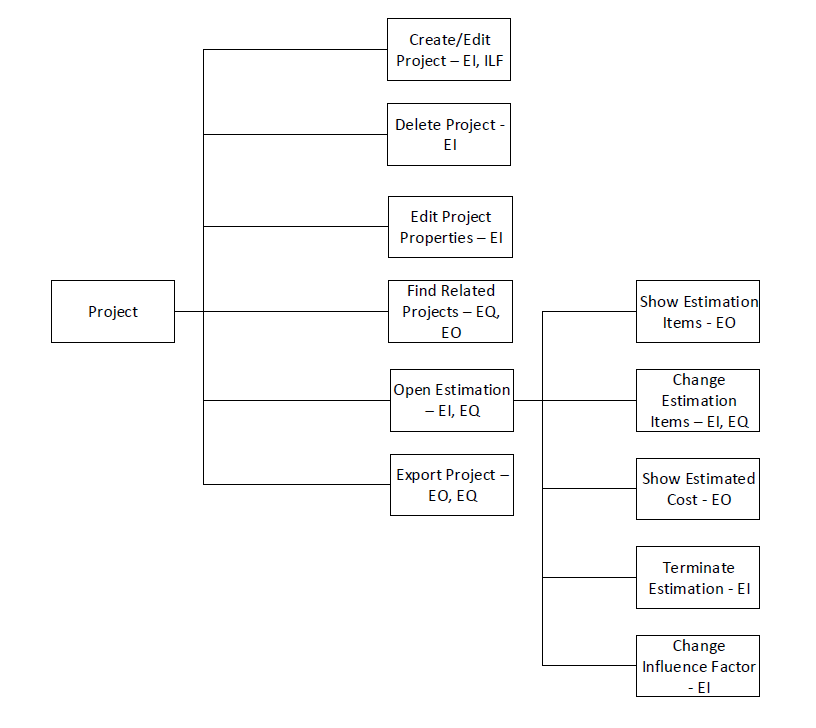
\includegraphics[width=14cm]{images/ScreenOverviewProject.PNG} 
	\caption{- Function Group - Project} 
	\label{fig:projectFunctionalityGroup}
\end{figure}
\begin{table}[h]
	\centering 
	\setlength{\tabcolsep}{4pt}
	\begin{tabular}{|l|c|c|c|c|}\hline
		Category		&  Amount 		&  Classification	&  Weight 	& Result of Row\\ \hline
		Input Data   	& 17      		& medium  			& 4			& 68	\\ \hline
		Request Data   	& 6      		& simple  			& 3			& 18	\\ \hline
		Output Data   	& 8      		& medium  			& 5			& 40	\\ \hline
		Dataset   		& 8      		& complex  			& 15		& 120	\\ \hline
		Reference Data  & 0      		& simple  			& 5			& 0	\\ \hline
		\textbf{Sum}   			&       		&   				& 			& \textbf{246}	\\ \hline
	\end{tabular} 
	\caption{Estimation - Total Points} 
	\label{estimation:data} 
\end{table}\\
As described in section \ref{FPMethod}, the next step is to set the influence factors which are described in table \ref{estimation:influence}. The influence factor \textit{Integration into other applications} is set to two because the application has no direct communication to other software. The application does not work with other applications but has local data, like the databases that have to be processed, which is the reason for setting the factor \textit{Local Data Processing} to two. As the application is only a local software for the end users device there is not much transaction to be excepted. To assure that there is enough time planned to implement an access to the database the factor \textit{Transaction Rate} is set to one. There are many algorithms and equations in the application which have to be checked for errors and exceptions. Also a high effort for the logical component is to be expected. Because of this all influence factors in the \textit{Processing Logic} group are set to the second highest value. For further development of the application a high effort has to be expected for \textit{Reusability} in the project which is the reason for this influence factor is set to two. There is not much data to be expected from other applications. Only the database causes a higher effort with queries to transform the data from the database in readable information for the application. Changes in the application can not be made by the user. He can change settings and some appearances which is why the influence factor \textit{Facilitate Change} is set to one. Calculated with the equation from \ref{FPMethod}, the influence factors result in a multiplier of \textbf{1.01}. Together with the \textit{total function points}, the influence multiplier is calculated with the equation \ref{fp:TFP} which has \textbf{243.54} points as result. Calculated with the points per day from table \ref{tab:pointsperday} the project is estimated to take \textbf{14} man days. In section \ref{result} it is analyzed how this estimation has worked out and how much time the project took in reality.\\
\begin{table}[h]
	\centering 
	\setlength{\tabcolsep}{4pt}
	\begin{tabular}{|l|c|}\hline
		Influence Factor						&  Weight 	\\ \hline
		Integration into other applications   	& 2      		\\ \hline
		Local Data Processing   				& 2      		\\ \hline
		Transaction Rate   						& 1      		\\ \hline
		Processing Logic   						&       		\\ \hline
		\phantom{ab}- Arithmetic Operation   					& 4      		\\ \hline
		\phantom{ab}- Control Procedure   					& 4      		\\ \hline
		\phantom{ab}- Exception Regulation   					& 8      		\\ \hline
		\phantom{ab}- Logic   								& 4      		\\ \hline
		Reusability   							& 3      		\\ \hline
		Stock Conversion  						& 2      		\\ \hline
		Facilitate Change   					& 1      		\\ \hline
		\textbf{Sum}   									& \textbf{31}      		\\ \hline
	\end{tabular} 
	\caption{Estimation - Influence Factors} 
	\label{estimation:influence} 
\end{table}

\section{Architecture}

The architecture of the project is described as a component diagram in fig. \ref{fig:components}. As usual in Android developments all resources are stored in the \texttt{resources} folder and are accessible from all other classes. The resources inherits \texttt{strings}, \texttt{images} and many more. Most used in the same folder is the \textit{Layout Data}, which inherits all information for displaying the user interface. Layout data is connected with the \textit{Activities} and \textit{Fragments} component which are responsible to display the user interface.\\
The \textit{Project Analyzer} component is responsible for collecting the data from all projects and putting them together for analysis. As the name says, \textit{Project Data} contains all informations for a single project. For reading and storing data to the database, the component \textit{Database Helper} allows simple \textit{Data Requests} and \textit{Data Insertions} to the database. It also allows a connection to the \textit{XML Helper} which reads data that is stored to XML files. The \textit{Project Exporter} component is called from an activity. It loads and compiles the data of a project for exporting it to files which can be used by external applications. Last component is the \textit{Project Relation Solver}. It gets an project from an activity and searches related projects in the database.

\begin{figure}[h] 
	\centering 
	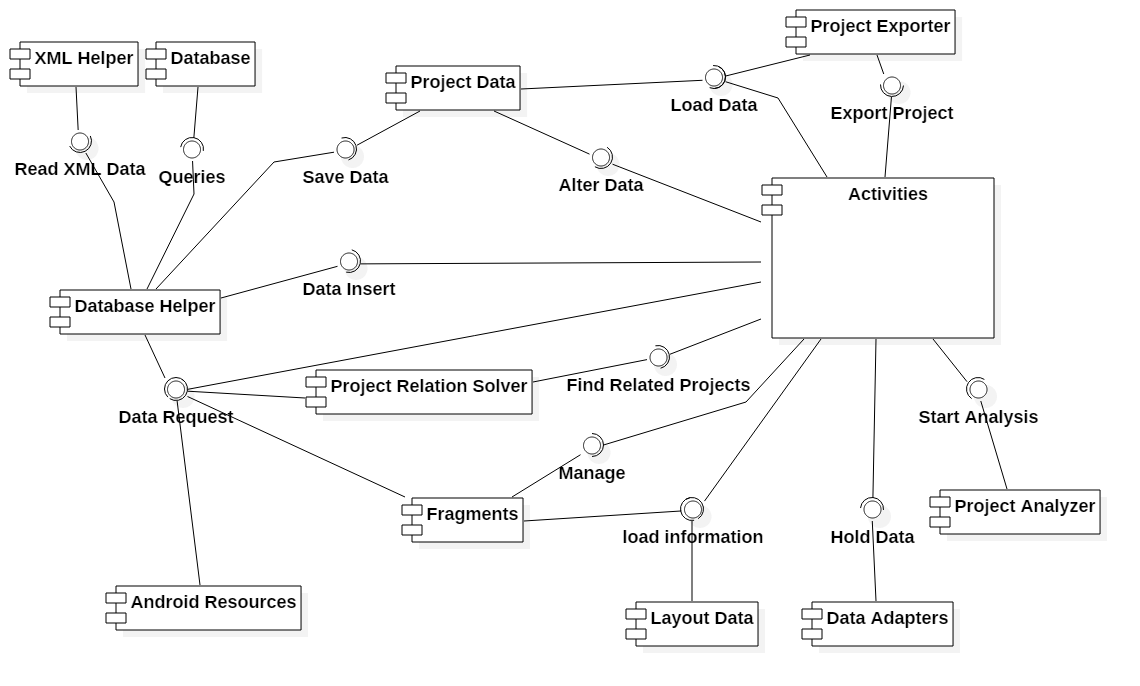
\includegraphics[width=14cm]{images/components.png} 
	\caption{- Component Diagram} 
	\label{fig:components}
\end{figure}

\section{Components}

This section explains the components from figure \ref{fig:components} in detail and what concepts they inherit. The concept of the component is described and examples are stated.

\subsection{Database Helper}

The \textit{Database Helper} component is responsible for accessing the database, where all project informations are stored. Every Class that needs access to the database should only create an object of this component and can read or write data to the database.\\
The component should contain name and path to the database and allow the initialization of the database. As described in fig. \ref{fig:sequenceDBHelper}, with the message \textit{Open Constructor}, an initialization of the database should be done in the constructor of classes that need access to it. This will opens the \textit{SQLite} database and ensures that request on the database can be performed and no error occurs while accessing a non initialized database. All functionalities that are working on the database are in fig. \ref{fig:sequenceDBHelper}, combined to the message \textit{Using Class} and combines the three categories, \texttt{SELECT}, \texttt{ALTER} and \texttt{DELETE}, for working with the database.\\ 
For requesting data from the database a Java class has to send a request with the table name and the selection criteria to the Database Helper. This will be transformed into a query which is send to the database. Before sending this data back to the calling Java class the database Helper has to transform the \textit{SQL} query result into readable information. Editing existing informations in the database is done with the message \textit{Alter Existing Data} and the parameters table name and data to be edited. Before sending data to the database the \textit{Database Helper} has to prepare it to insert them in the right column of the table. This query will return true if inserting was successful and false if it was not. Last message option is \textit{Delete Data} which will delete entries from the database. The parameter \textit{tablename} and \textit{Data ID} are the identifiers for a selected entry. Before deleting data from the database the \textit{Database Helper} has to check if there are any other tables depending to the selected entry and has to ensure that they are deleted too if necessary. After all depending tables are identified the Database Helper will send the delete query to the database. It will then return a boolean value for the deletion process which is forwarded to the Java Class.
\begin{figure}[h] 
	\centering 
	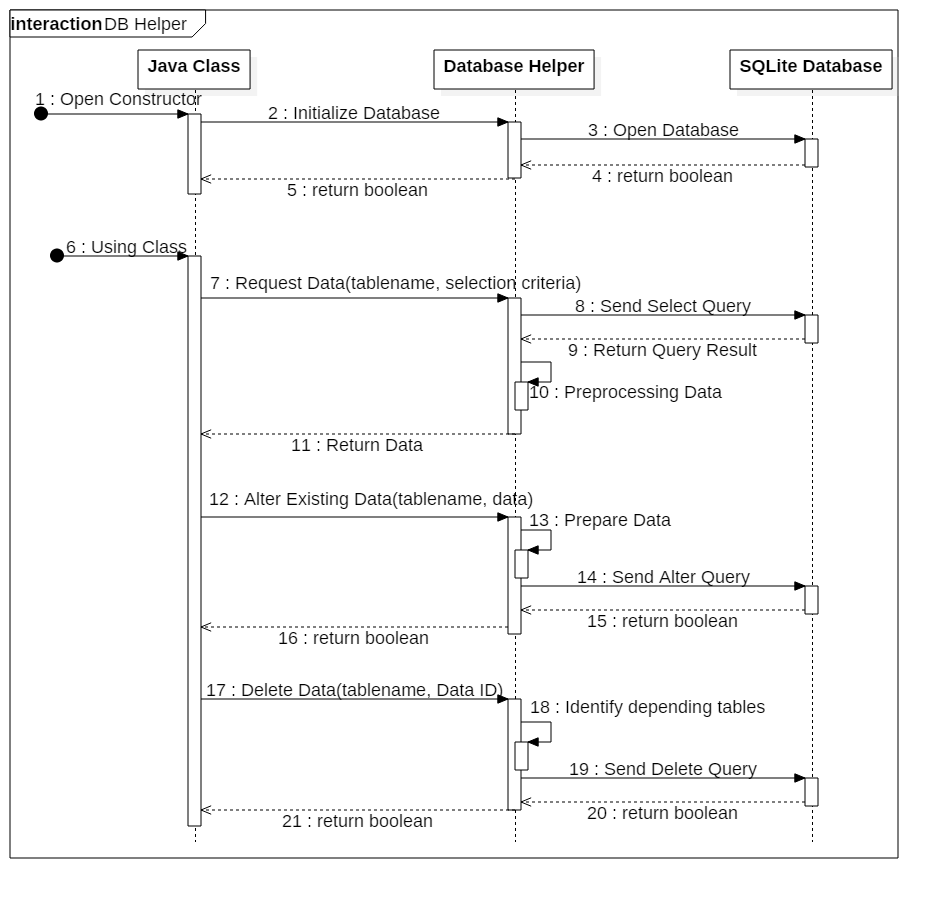
\includegraphics[width=14cm]{images/DBHelper.png} 
	\caption{- DB Helper Sequence Model} 
	\label{fig:sequenceDBHelper}
\end{figure}
\subsection{Project Data}

The \textit{Project Data} component was created to combine all data of a project from the database and make it accessible for other classes. It contains \textit{Name}, \textit{Description}, \textit{Creation Date} and \textit{Estimation Technique} at the first level of the component. This makes it possible to get a fast overview of the different projects in the application. For estimation specific purposes the \textit{Estimation Items} and \textit{Influence Factor} are minor components for the project data and differ from the projects estimation technique. The \textit{Properties} are also a minor component to build a module-based structure. As the output information of estimation techniques is the same, the main component contains the amount of \textit{Estimated Man Days} for the project. If the project is completed the \textit{Final Man Days} represent the time the project really took. This value is important to improve future estimations as described in section \ref{adjustedEstimationProcess}, where the improvement process is specified.
\begin{figure}[h] 
	\centering 
	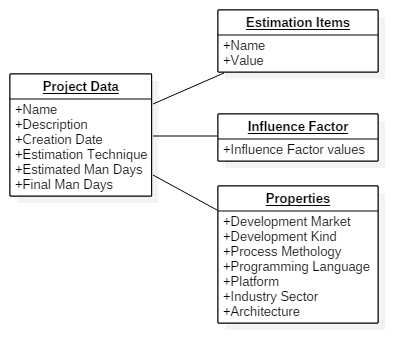
\includegraphics[width=10cm]{images/ObjectDiagramProject.png} 
	\caption{- Object Diagram for Projects} 
	\label{fig:objectDiagrammProject}
\end{figure}

\subsubsection{Project Properties}

This minor component contains the information that is needed for the \textit{Project Relation Solver} in section \ref{projectRealtionSolver}. It is a data component which stores all properties that allows reading and editing. Access to the properties is granted only through the project component which assures that a property is bound to a project.\\
The available properties are based upon the parts a project can be split to. Not every available factor of a project makes sense for categorizing it. For example a categorization into the size of the project makes no sense as this cannot be compared to a project that is not estimated or developed. Also a categorization of the costs makes no sense as it cannot be compared to a project that has to be estimated. For this reason the available properties are \textit{Development Market}, \textit{Development Type}, \textit{Procedure Model}, \textit{Platform}, \textit{Industry Sector}, \textit{Programming Language} and \textit{Software Architecture}. These values categorize a project without saying something about the size or cost and makes it possible to compare with other projects.\\
All project properties contain only a selection of the possible values as a showcase. For each category further options are possible. Properties that have more options that are not implemented at the moment these are combined in the option \textit{other}. But this option is always calculated with the highest possible distance at the moment. It should only illustrate that there are more options possible and allow a selection if the needed property is not available.
\subsubsection{Estimation Items}

All items for the estimation are in the \textit{Estimation Items} components. These are the items for an estimation technique that are responsible for the estimation itself. In the \textit{Function Point} estimation for example, these items calculate the value \textit{E1} from the equation \ref{fp:E1}.

\subsubsection{Influence Factors}

This component contains all informations for \textit{Influence Factors}. These are \textit{name}, \textit{chosen value} and the \textit{limit} for the value. This component is also responsible for preprocessing the influence factor for usable information at the calculation of the estimation. In the Function Point estimation for example, this component calculates the value \textit{E2} and \textit{E3} that are described in section \ref{fp:classificationInfluence}.

\subsection{Function Point Estimation}

This component is responsible for estimating a project with the function point technique. It inherits the calculation from section \ref{FPMethod} and calculates the estimated man days. To get the best calculation of man days the component searches all existing projects in the database that are already terminated and are using the function point technique. In all of these projects the component searches for the project with highest total function points that are less then the selected project and for the lowest total function points that are higher than the selected project. Next step is to calculate the points per day from these projects with the equation \ref{pointsday}. If there is no project available for one or both of these value the component will instead take the base points per day value from table \ref{tab:pointsperday}.
\begin{equation}
\textit{Points per Day} =  \frac{\textit{Total Function Points}}{\textit{Final Man Days}}\label{pointsday}
\end{equation}
With these two values the component will then calculate the average point per days which is then used to calculate the man days of the actual project.

\subsection{Project Relation Solver}\label{projectRealtionSolver}

To fulfill the goal \textit{G06} from section \ref{objectives}, this component is responsible to find related project. The point of this component is to compare already existing projects with a selected one. This should help the user to get an overview of how similar projects were estimated. Furthermore the \textit{Project Relation Solver} should allow to transfer the estimation from a related project to the selected to have an estimation where the user can build on.\\
The \textit{Project Relation Solver} compares a selected project with every other available project from the database. This comparison is made in mainly three steps \textit{determination of the property distances}, \textit{determination of the total distance} and \textit{calculation of the relation}.

\subsubsection{\textbf{Determination of the Property Distances}}
Each project has eight different properties which are crucial for finding a relation. These properties are \textit{Development Market}, \textit{Development Kind}, \textit{Procedure Model}, \textit{Platform}, \textit{Industry Sector}, \textit{Programming Language} and \textit{Software Architecture} and the \textit{Estimation Technique}. The first step for calculating the project relation is to compare each property and get the distance. Each of them has its own calculation for the distance and a different weight to fit in the \textit{total distance} equation. 

\paragraph*{\textbf{Estimation Technique}}

The selected estimation technique will influence the relation between projects. As it should be possible to transfer the estimation from a related project, this feature is not possible if these projects do not use the same estimation technique. So it is an important factor for the calculation. If the estimation techniques are equal the value for the distance is \textit{0}. If it are different this value is \textit{1}.

\paragraph*{\textbf{Development Market}}
The \textit{Development Market} property stands for the target market of a project and has three possible options: \textit{Inhouse Development}, \textit{Customer Development} and \textit{Anonymous Market}. To calculate the distance between development markets it was analyzed for whom the project is developed, what is the main factor for the budget, how high the risk of development is and how predictable profit is.\\ 
The \textit{Inhouse Development} is for developing projects inside the company. They are usually have the same procedure as other projects despite the fact that they don't yield a profit and have a low risk of development and a fixed budget. In the \textit{Customer Development} the risk depends on the customer needs but are predictable. Profit is to be expected high and is connected with the project budget. By \textit{Anonymous Market} developments a high risk is to be expected. Regardless of market analysis it is unsure that the project will be a success and generate profit. The budget for this market type is set from the company itself.\\
All distances between these markets are described in table \ref{property:devmarket} and are based on the above description. For example, the development for a customer is quite similar to an anonymous market development, so the distance between those is set to one. The big difference is that the profit is unsure for the anonymous market development. When comparing similar markets to each other the distance is zero as they are the same.
\begin{table}[h]
	\centering 
	\setlength{\tabcolsep}{4pt}
	\begin{tabular}{|l|l|c|}\hline
		Development Market		& Compared to 			&  Distance 	\\ \hline
		Inhouse Development   	& Customer Development	& 2      		\\ \hline
		Customer Development   	& Anonymous Market 		& 1      		\\ \hline
		Anonymous Market   		& Inhouse Development 	& 3     		\\ \hline
	\end{tabular} 
	\caption{Development Market - Distance} 
	\label{property:devmarket} 
\end{table}
\paragraph*{\textbf{Development Type}}
Different \textit{Development Types} describe the main reason for the project. A \textit{New Project} is developed if there is no previous project to build on or is a new conceptual formulation with no experiences so far. An \textit{Extension Project} is made for expansion of existing software from previous projects. The third type are \textit{Research Projects}, which are usually made to test an idea or to create a prototype for an analysis. These development types can be differentiated in the \textit{main goal} of the project, \textit{customer} and \textit{profit level}. To introduce this differentiation the profit level describes the expected money and is divided into values from zero to two. \textit{Zero} declines that the project does not generate any profit. The value \textit{one} expects medium profit and \textit{two} expects a high profit for the project.\\
The distances described in table \ref{property:devtype} are based on the above descriptions. A comparison between new projects and research project has the distance two. A research project does not generate any profit and has a different target than a new project. The same applies with the comparison of an extension project with a research project. By comparing a new project to an extension project the distance is set to one because the expected profit is smaller than in a new project. The reason for this is that an extension project builds up on a previous project and is an addition to a previous contract which normally get a smaller budget.\\
\begin{table}[h]
	\centering 
	\setlength{\tabcolsep}{4pt}
	\begin{tabular}{|l|l|c|}\hline
		Development Type		& Compared to 			&  Distance 	\\ \hline
		New Project   			& Research Project		& 2      		\\ \hline
		Extension Project   	& New Project 			& 1      		\\ \hline
		Research Project   		& Extension Project 	& 2     		\\ \hline
	\end{tabular} 
	\caption{Development Market - Distance} 
	\label{property:devtype} 
\end{table}
\paragraph*{\textbf{Procedure Model}}
The next property is the used procedure model. There are six procedure models for selection available. The distance in table \ref{property:proceduremodel} is calculated by differentiating each procedure by \textit{model type}, \textit{suitable team size}, \textit{formalization}, \textit{industry focus} and \textit{process cover}. \textit{Model type} simply splits the procedure models in sequential and iterative types. The \textit{suitable team size} indicates the laid out size of team members are useful for this model, which means with how much people this model can be used effectively. \textit{Formalization} indicates how much has to be put into the documentation of the process steps. \textit{Process cover} describes if the procedure model involves all main project processes, which are \textit{development}, \textit{test project management}, \textit{quality assurance} and \textit{change management} \cite{incom}.\\
For example the V-Model is a sequential model for small and large teams. It is under a strong formalization pressure and covers all main project processes. It is used in all industry sectors and is strongly represented in sectors with high standards and formalization requirements such as the pharmacy industry. Scrum is an iterative model which is used for small teams. It does not cover all processes. Testing and quality assurance are not part of the scrum process. Scrum has no specific industry sector and is represented in different industries. With this differentiation the distance is 5, which is also described in table \ref{property:proceduremodel}. The other distances are calculated the same way. A comparison between all available procedure models can be found in the appendix XXX.
\begin{table}[h]
	\centering 
	\setlength{\tabcolsep}{4pt}
	\begin{tabular}{|l|l|c|}\hline
		Procedure Model			& Compared to 	&  Distance 	\\ \hline
		Scrum   				& V-Model		& 5      		\\ \hline
		Waterfall Model   		& V-Model 		& 3      		\\ \hline
		Spiral Model   			& V-Model 		& 4     		\\ \hline
		Iterative Development   & V-Model 		& 4     		\\ \hline
		Prototyping  			& V-Model 		& 6     		\\ \hline
	\end{tabular} 
	\caption{V-Model - Distance} 
	\label{property:proceduremodel} 
\end{table}

\paragraph*{\textbf{Platform}}
Platform is the property that describes where the implemented software is deployed. The difference between platforms is calculated with the porting costs from one platform to another. This costs are the \textit{main programming language} of the platform, \textit{quality assurance}, \textit{OS family} and the \textit{deployment difficulty}. Main programming language is the language that has the biggest portion by developing software for a platform. Quality assurance means the effort that has to be done for testing the developed project for a platform and \textit{OS family} describes the family on which the platform is based on. The deployment difficulty describes the effort that has to be taken for projects to be installed.\\
For example the main programming language for \textit{Android} is \textit{Java}. Quality assurance has to be done with much effort as there are many different devices that support Android and is a member of \textit{Unix-like} operating systems. The deployment effort is very low. An \textit{Android} application is packed as as \textit{.apk}-file which will be installed automatically on a device. For \textit{iOS} the main programming languages are \textit{Objective-C} and \textit{Swift}. The selection of devices is limited but the quality assurance is although at high effort because \textit{Apple} has high restrictions for software. It also belongs to the \textit{Unix-like} operating systems and it is more difficult to deploy software to devices. It is needed to have an developer account for testing software on the device and it is not possible to install software without the \textit{App-Store}. This distance and the distance of Android to all other available platforms is described in table \ref{property:platform}.
\begin{table}[h]
	\centering 
	\setlength{\tabcolsep}{4pt}
	\begin{tabular}{|l|l|c|}\hline
		Platform			& Porting to 	&  Costs 	\\ \hline
		Android   			& iOS					& 4      		\\ \hline
		Android   			& Windows Phone 		& 3      		\\ \hline
		Android   			& Mac OS 				& 5     		\\ \hline
		Android   			& Linux 				& 4     		\\ \hline
		Android  			& Windows 7 			& 5     		\\ \hline
		Android  			& Windows 8				& 5     		\\ \hline
		Android  			& Windows 10 			& 5     		\\ \hline
		Android  			& Windows Universal App	& 6     		\\ \hline
		Android  			& Web Development 		& 5     		\\ \hline
		Android  			& Other 				& 7     		\\ \hline
	\end{tabular} 
	\caption{Platform - Porting cost} 
	\label{property:platform} 
\end{table}

\paragraph*{\textbf{Industry Sector}}
The distance for industry sector is not calculated with an equation as it is mostly an empiric property. It simply compares if the selected sectors are equal or not. If the industry sector does not apply to one of the available sectors there is the option to select \textit{Other} as sector. For the calculation the distance between industry sectors is set to \textit{zero} if they are equal and  \textit{one} otherwise. The available options for this property are:
\begin{itemize}
	\item \textit{Agriculture}
	\item \textit{Automotive}
	\item \textit{Banking}
	\item \textit{Bars and Restaurants}
	\item \textit{Business Service}
	\item \textit{Construction}
	\item \textit{Education}
	\item \textit{Electronics}
	\item \textit{Entertainment}
	\item \textit{Finance}
	\item \textit{Health}
	\item \textit{Internet}
	\item \textit{Music Production}
\end{itemize}

\paragraph*{\textbf{Programming Language}}\label{section:ProgrammingLanguage}
The Programming Language describes the main language for the project. As an example for the platform Android the main programming language would be Java. This Property has the most values for calculating the distance between two options. It is divided in two parts. \textbf{Part one} is calculating distance on the basis of programming language properties as described by Ruknet \cite{ruknet}. He categorized the programming languages with 12 different properties:
\begin{enumerate}
	\item \textbf{Imperative}\\ This value focuses in describing how a program operates. It simply exists on a sequence of instruction.
	\item \textbf{Object Oriented}\\ This Property describes if the language supports the concept of objects.
	\item \textbf{Functional}\\ These property is a programming paradigm that treats computation as the evaluation of mathematical functions. 
	\item \textbf{Procedural}\\ This programming paradigm allows routines and subroutines and contains a series of computational steps.
	\item \textbf{Generic}\\ Generic programming is a style which allows algorithms to be written in terms of types \textit{to-be-specified-later} that are then \textit{instantiated} when they are needed.
	\item \textbf{Reflective}\\ This is the ability of a programming language to examine and modify its own structure and behavior.
	\item \textbf{Event-Driven}\\ An event-driven programming language is determined by events such as user actions or messages from other programs.
	\item \textbf{Failsafe}\\ The ability to throw exceptions if an operation or other system calls fails.
	\item \textbf{Type Safety}\\States if a programming language discourages or prevents type errors which are stated in the values \textit{safe} and \textit{unsafe}.
	\item \textbf{Type Expression}\\ This property describes if the programmer must explicitly associate each variable with a particular type.
	\item \textbf{Type Compatibility}\\ This implies the use of a type checker in the programming language which verifies if an expression is consistent with the expected type by the context in which that expression appears.
	\item \textbf{Type Checking}\\ A process of verifying and enforcing the constraints of types at run-time or compile time.\\
\end{enumerate}
Each property is converted to a numerical representation form which represents each of the possible values. For most of the properties this is simple as the possible values are \textit{true} or \textit{false} which are represented as \textit{1} and \textit{0} in table \ref{property:proglang}. Four values can not be distinguished in true or false. For failsafe, these values are \textit{safe}, \textit{unsafe} and \textit{unknown}. In the case of \textit{failsafe} the value \textit{0} means unknown, \textit{1} is unsafe and \textit{2} means safe. Type expression has also three values which are implicit, explicit an unknown. Implicit is represented as \textit{1}, explicit as \textit{2} and unknown as \textit{0}. The three values for type compatibility are nominal, structural and not stated. These values are also represented as 1 for nominal, 2 for structural and 0 for not stated. The last property with more options is type checking. It can separated in \textit{static}, \textit{dynamic} and \textit{unknown}. These are represented as \textit{1} for \textit{static} and \textit{2} for \textit{dynamic}. \textit{Unknown} is as in the properties before represented as \textit{0}.\\
This allows a calculation of the \textit{Distance} of two programming languages. As this is calculated with the absolute value of each category. The constant \textit{c} is the amount of all categories, which is twelve. For each category \textit{$K_i$} of the compared programming language, the value of the other language is subtracted. This summed up is the distance of these two languages.
\begin{equation}
\textit{Distance} = \sum \limits_{i=1}^c \lvert K_i - K'_i\rvert \label{pl:distanceequation}
\end{equation}
Table \ref{property:proglang} describes the comparison between C++ and Java as an example. Those two programming languages only differ in two categories, namely reflective and failsafe. To calculate the distance for those two languages the differnce between these categories is calculated with the equation from \ref{pl:distanceequation}. The result is a distance of 3.\\
\begin{table}[h]
	\centering 
	\setlength{\tabcolsep}{4pt}
	\begin{tabular}{|l|c|c|c|c|c|c|c|c|c|c|c|c|}
		\multicolumn{1}{c}{\textbf{Programming Language}}& \multicolumn{1}{c}{\rotatebox{90}{imperative} }&  \multicolumn{1}{c}{\rotatebox{90}{object oriented}} &  \multicolumn{1}{c}{\rotatebox{90}{functional}}&  \multicolumn{1}{c}{\rotatebox{90}{procedural}}& \multicolumn{1}{c}{\rotatebox{90}{generic}}&  \multicolumn{1}{c}{\rotatebox{90}{reflective}}& \multicolumn{1}{c}{\rotatebox{90}{event driven}}&  \multicolumn{1}{c}{\rotatebox{90}{failsafe}}&  \multicolumn{1}{c}{\rotatebox{90}{type safety}}&  \multicolumn{1}{c}{\rotatebox{90}{type expression}}&  \multicolumn{1}{c}{\rotatebox{90}{type compatability}}&  \multicolumn{1}{c}{\rotatebox{90}{type checking}}\\ \hline
		C++   				& 1& 1 & 1 & 1& 1& 0& 0& 0& 1& 2& 1& 1    		\\ \hline
		Java   				& 1& 1 & 1 & 1& 1& 1& 0& 2& 1& 2& 1& 1    		\\ \hline
	\end{tabular} 
	\caption{Programming Language - Distance} 
	\label{property:proglang} 
\end{table}\\
The \textbf{second part} is calculating conversion cost in another language which is the estimated effort for converting the source code. These are calculated with the equation \ref{pl:conversioncosts}, which estimates the cost factor for a conversion. These costs are simplified as the \textit{Amount} of different categories plus an constant effort factor of one. This equation should illustrate that each different category generates effort for transforming the source code. It has to be adapted for different code paradigms and functionalities. \\
\begin{equation}
\textit{Conversion Costs} = \textit{Amount} + 1\label{pl:conversioncosts}
\end{equation}\\
In the case of a conversion between C++ an Java we have an amount of different columns of \textit{2}. Summed with the constant cost factor from the equation the conversion costs, as described in table \ref{property:proglangconversion}, are \textit{3}.\\
\begin{table}[h]
	\centering 
	\setlength{\tabcolsep}{4pt}
	\begin{tabular}{|l|l|c|}\hline
		Programming Language	& Converting to &  Distance 	\\ \hline
		Java   				& Cpp		& 3      		\\ \hline
	\end{tabular} 
	\caption{Programming Language - Conversion Cost} 
	\label{property:proglangconversion} 
\end{table}\\
To get a total distance between two programming languages, the distance and conversion costs are summarized, as described in equation \ref{pl:totaldistance}. In the example of C++ and Java we have a distance of \textit{3} and conversion costs of \textit{3} which results in a total distance of \textit{6}.
\begin{equation}
\textit{Total Distance} = \textit{Distance} + \textit{Conversion Costs}\label{pl:totaldistance}
\end{equation}\\
The available languages for this property are \textit{C}, \textit{C\#}, \textit{C++}, \textit{COBOL}, \textit{Clojure}, \textit{Java}, \textit{Javascript}, \textit{Matlab}, \textit{Objective-C},\textit{ PHP}, \textit{Prolog}, \textit{Python} and \textit{Scala}. The complete categorization and converting costs of all programming languages can be found in the appendix XXX.

\paragraph*{\textbf{Software Architecture}}
Software Architecture describes the high level structure of a software system and includes software elements, relations among them, and properties of both elements and relations. This property set the architecture of the project. It allows a differentiation on the fundamental structural choices which is important as it is costly to change a once implemented architecture.\\
The available options are \textit{client-server}, \textit{event driven}, \textit{layered}, \textit{microkernel}, \textit{microservices}, \textit{model view controller}, \textit{serviceoriented} and \textit{space based architecture}. These architectures are categorized with the help of architecture patterns as described by Richards \cite{archpatterns}. He analyzed software architectures by classifying them into \textit{overall agility}, \textit{ease of deployment}, \textit{testability}, \textit{performance}, \textit{scalability} and \textit{ease of development}. These are the categories in which a software architecture can be divided into. Each of the values is stated with \textit{low}, \textit{medium} or \textit{high}. These values are represented in the table and database as \textit{1}, \textit{2} or \textit{3}.\\
\begin{itemize}
	\item \textbf{Overall Agility}\\Describes the ability to respond to a constantly changing environment.
	\item \textbf{Ease of Deployment}\\Describes the deployment process and how changes affect deployment.
	\item \textbf{Testability}\\The way of how the architecture can be tested.
	\item \textbf{Performance}\\The ability a pattern can be lend to high-performance applications.
	\item \textbf{Scalability}\\Scalability describes how good the application with this pattern can be scaled.
	\item \textbf{Ease of Development}\\This describes the complexity for implementing the architecture.\\
\end{itemize}
Each software architecture can be differentiated with these properties. Another distinguishing feature is the \textit{category}. Possible values are \textit{distributed}, \textit{interactive}, \textit{adaptive} and \textit{mud-to-structure}. The category is distinguished with an equality verification. Table \ref{property:architecture} describes the categorization of \textit{layered} and \textit{eventdriven} pattern as an example. The categorization of all available patterns can be found in the appendix XXX.\\
The \textit{layered architecture} is the de facto standard for most \textit{Java} applications and therefore is widely known by most architects, designers, and developers. It is time-consuming to make changes in this architecture pattern because of the monolithic nature of most implementations and one small change to a component can require a redeployment of the entire application. The pattern can be easily tested by mocking or stubbing layers. As some layer applications may run well, the pattern itself is not a high-performance architecture, also scaling applications with this pattern is hard due to different layers. Because this pattern is well known and not overly complex to implement the ease of development is considered as high.\\
The \textit{eventdriven architecture} is a distributed asynchronous architecture pattern used to produce high scalable applications. Changes are generally isolated to one or a few event processors and can be made quickly without impacting other components. It tends to be easier in this architecture deploy than the mediator topology, primarily because the event mediator component is tightly coupled to the event processors. Testing is complicated because of the asynchronous nature of this pattern. The pattern achieves high performance through its asynchronous capabilities. Scalability is naturally achieved in this pattern through highly independent and decoupled event processors. Development can be complicated due to the asynchronous nature of the pattern as well as contract creation and the need for more advanced error handling conditions. The properties of the described patterns are visualized in table \ref{property:architecture}.\\
To calculate the distance between these two architectures, each property of the architecture will be subtracted with the property from the other architecture as described in equation \ref{archdistance}. This calculation is the same as the distance for the programming languages. For the different categories the value \textit{1} is added if they are not equal and \textit{0} if they are. 
\begin{equation}
\textit{Architecture Distance} = \sum \limits_{i=1}^c \lvert P_i - P'_i\rvert\label{archdistance}
\end{equation}\\
In the case of the comparison of \textit{layered architecture} and \textit{eventdriven architecture}, as described in \ref{property:architecture}, the result of the distance calculation is 12. As the categories are not equal the value 1 is added to the distance which results in a total distance of 13 for these two patterns.
\begin{table}[h]
	\centering 
	\setlength{\tabcolsep}{4pt}
	\begin{tabular}{|l|c|c|c|c|c|c|c|}
		\multicolumn{1}{c}{\textbf{Software Architecture}}& \multicolumn{1}{c}{Category }&  \multicolumn{1}{c}{\rotatebox{90}{overall agility}} &  \multicolumn{1}{c}{\rotatebox{90}{ease of deployment}}&  \multicolumn{1}{c}{\rotatebox{90}{testability}}& \multicolumn{1}{c}{\rotatebox{90}{performance}}&  \multicolumn{1}{c}{\rotatebox{90}{scalability}}& \multicolumn{1}{c}{\rotatebox{90}{ease of development}}\\ \hline
		Layered Architecture   		& distributed& 1& 1 & 3& 1& 1& 3   		\\ \hline
		Eventdriven Architecture	& interactive& 3& 3 & 1& 3& 3& 1    		\\ \hline
	\end{tabular} 
	\caption{Software Architecture - Distance} 
	\label{property:architecture} 
\end{table}

\subsubsection{\textbf{Determination of the Total Distance}}
After determining the distance for each property the next step is calculating the total distance of two projects with the equation \ref{totaldistance}. Each property has to be multiplied with the weight from table \ref{propertyweights}, which sets distances with lower value the same importance as high distances. It also allows a prioritization of the different values. 
\begin{equation}
\textit{Total Distance} = \sum \limits_{i=1}^n ( D_i \cdot Weight_i )\label{totaldistance}
\end{equation}
The max distance of the programming languages is \textit{28}, for example, whereas the highest value of the development type distance is \textit{2}. To set more importance in the development type value this property is multiplied with \textit{3}.
\begin{table}[h]
	\centering 
	\setlength{\tabcolsep}{4pt}
	\begin{tabular}{|l|c|}\hline
		Property	& Weight 	\\ \hline
		Estimation Method   	& 1      	\\ \hline
		Development Market   	& 2      	\\ \hline
		Development Type   		& 3      	\\ \hline
		Procedure Model   		& 2      	\\ \hline
		Platform   				& 1.5      	\\ \hline
		Industry Sector   		& 1      	\\ \hline
		Programming Language   	& 1      	\\ \hline
		Software Architecture   & 1      	\\ \hline
	\end{tabular} 
	\caption{Property Weights} 
	\label{propertyweights} 
\end{table}
\subsubsection{\textbf{ Calculation of the Relation}}
The last step is calculating the relation of projects with the total distance from equation \ref{totaldistance}. As the distance of the properties does not describe the relation but the difference between two projects, this is calculated with the equation \ref{relation}. The \textit{Max} value is the maximum possible total distance plus an addition of \textit{10}. This should assure that two projects are never totally equal, because if they are equal they are the same and there is no need for creating a new project. This value describes the minimum difference of projects as 10\%. The maximum distance between projects is \textit{93}, so the \textit{Max} value for the calculation is \textit{103}. To get the relation this \textit{Percentage Difference} has to be subtracted from 100\%. The result of this equation is the percentage relation of two projects and allows to find related estimation to give the user an overview of previous projects.\\
\begin{equation}
\textit{Percentage Relation} =  100 - (\frac{\textit{Total Distance}}{\textit{Max}})\cdot 100\label{relation}
\end{equation}
\subsubsection{\textbf{Example Calculation}}

To illustrate this calculation this sections describes a sample calculation with the project properties from table \ref{exampleproperty}. As described above, the first step is calculating the distance of each property. These distances calculated with the equation \ref{totaldistance} and the weights from table \ref{propertyweights} result into a total distance of \textit{23.5}. Next step is to calculate the percentage relation with equation \ref{relation}, which results into a relation of \textbf{77.18\%} of both projects.
\begin{table}[h]
	\centering 
	\setlength{\tabcolsep}{4pt}
	\begin{tabular}{|l|c|c|c|}\hline
		\phantom{abc}	& \textbf{Project A}	& \textbf{Project B} 	& \textbf{Distance}\\ \hline
		Estimation Technique   	& Function Point  & Function Point   & 0 	\\ \hline
		Development Market   	& Anonymous Market & Inhouse Development &3     	\\ \hline
		Development Type   		& New Project & New Project    	& 0\\ \hline
		Procedure Model   		& Scrum  & Scrum    	& 0\\ \hline
		Platform   				& Android & Windows Phone  &3   	\\ \hline
		Industry Sector   		& Education  & Internet     &1	\\ \hline
		Programming Language   	& Java  & C++    	&6\\ \hline
		Software Architecture   & Model View Controller  & Client-Server    	&4\\ \hline
	\end{tabular} 
	\caption{Example Project Properties} 
	\label{exampleproperty} 
\end{table}\newpage

\subsection{Project Analyzer}

The task of this component is to show how the estimations changed over time. It should show each project with the \textit{estimated days} and the \textit{final days}. Depending on the estimation technique the analysis should show the amount of the estimation. The analysis is visualized in diagram \ref{fig:analysis}. It should help visualizing the progress of the estimation. As with further estimations, the gap between the estimated days and the final days should become smaller.If the diagram shows project with a high gap between the final man days and the estimated man days it means that the estimation was not precise enough.
\begin{figure}[h] 
	\centering 
	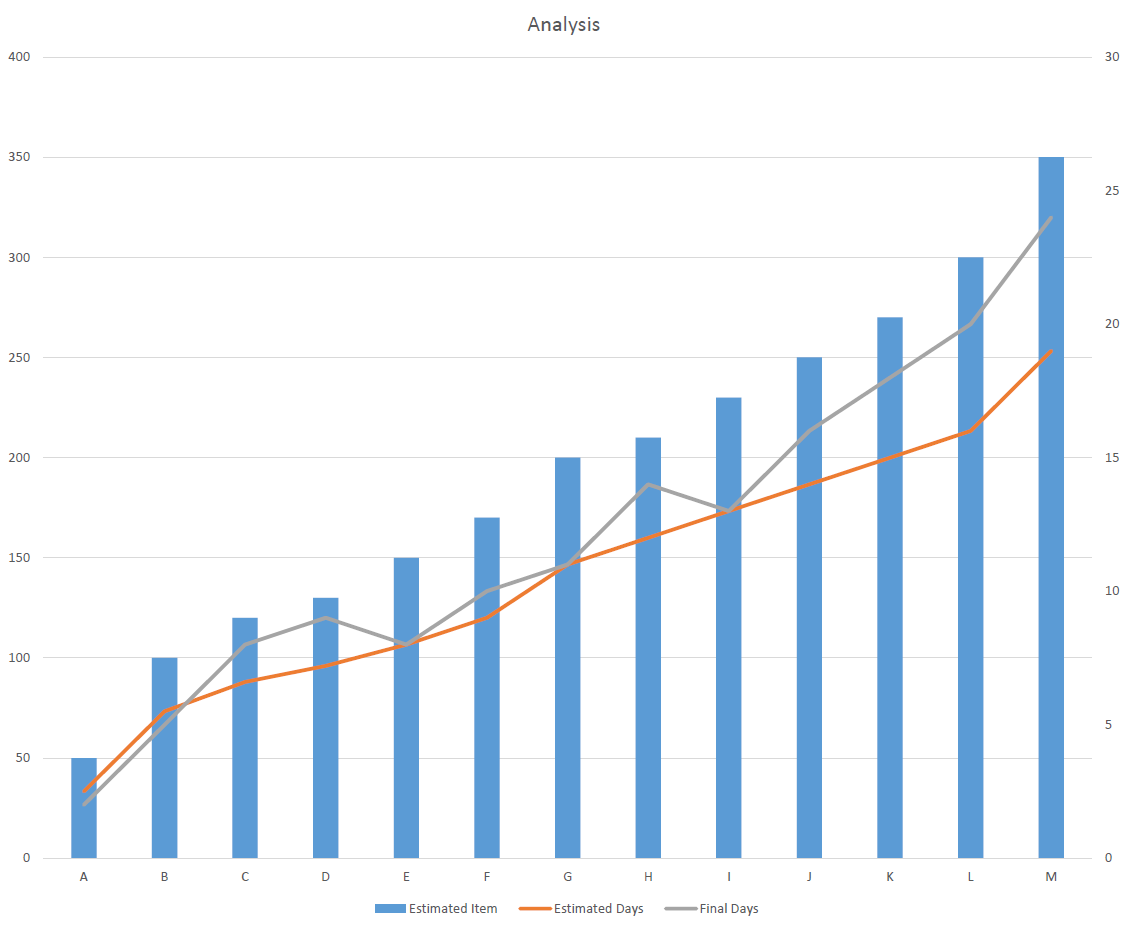
\includegraphics[width=12cm]{images/analysis.png} 
	\caption{- Analysis Diagram} 
	\label{fig:analysis}
\end{figure}

\subsection{Minor Components}

Beside the main components their are some minor components which are not essential but are mentioned here.

\subsubsection{\textbf{Export}}

The \textit{Export} component is responsible for preparing a project as a table which should allow further processing of the estimation. All items of the estimation will be transformed to an excel sheet according to the estimation technique. Also all properties of the project will be exported to the file. This allows printing the estimation or sending it via e-mail.

\subsubsection{\textbf{Accessing Resources}}\label{accessingresources}

To implement a multilingual option for data from the database this component should do the essential work. All values of data strings are stored in the database as \texttt{'<NAME>\_string'}. This value is also stored in the string resource file of Android and is connected to the string value in the device language. These files already support multilingualism which means that this component only needs to build a connection between the resource files and the database value.\\
If a value from the database is queried, the component will look for the name in the resource files. The right value in the device language will then be returned as a string. To add a string id from the database to a new entry the process works exactly the same in the other direction. The component searches for the belonging id of a string. The id is the representation of resources in Android which are newly generated after each start of the application and have to be managed in the component. This id is linked to the database string value and allows queries of the \textit{Database Helper} component. 

\subsubsection{\textbf{Project Filter}}

The Project Filter helps to maintain an overview of all projects. It is an addition to the \textit{Project Overview} which allows restriction of the displayed projects. Deleted projects will not be displayed by default, which can be set with the filter. Another possible option is to display only projects of a specific estimation technique. This component is held modular, so it is simple to add new parameters for filtering the projects. 

\subsubsection{\textbf{Help Articles}}

The \textit{Help Articles} allow the user to inform them self about the functionalities of the application and fundamentals like \textit{Function Point}. This should be a guide for new and unexperienced users.\\
All Articles are stored in an \texttt{XML} file which will be synchronized with the server in a later version of the application. The component is responsible for reading all articles from this file and allow the application to display them. These articles are not stored in the database as if they may have any desired length and must be available in different languages. 
 
\subsubsection{\textbf{Project Analyzer}}

This component evaluates all project data and delivers an overview in the form of diagrams. Figure \ref{fig:statistic} is an example of such an overview. This statistic shows how many projects used which programming language as their property. Purpose of this is to help users an overview of how often properties are used.

\begin{figure}[h] 
	\centering 
	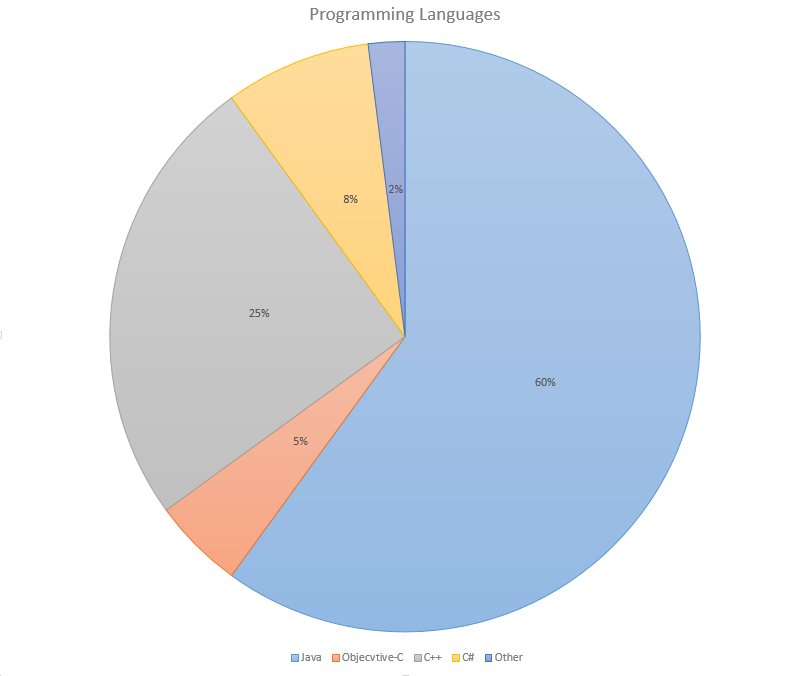
\includegraphics[width=14cm]{images/percentage.png} 
	\caption{- Use of Programming Languages} 
	\label{fig:statistic}
\end{figure}

\section{Database design}

This section introduces the design of the databases. To allow using a filled database in the application, without creating it with \textit{SQL} commands during the first start, the database was designed and filled before the implementation. The process of accessing an existing database is described in section \ref{exDB}. Their are two separated databases in the application. The \textit{Project Database}, which inherits all informations about projects, estimations and properties, and the \textit{Userinformation Database}, which is designed for a further use with a server and inherits user informations and server messages.\\

\subsection{Project Database}

The \textit{Project Database} is the main storage component in the application. It contains all important informations for the \textit{Project Relation Solver} and possible values for selecting \textit{Estimation Method} and \textit{Properties}. All created projects and influence factors will be stored here and allow a consistent processing. All tables must have a primary key column which is called \textit{\_id} or otherwise this table is not recognized by Android. Also the table \textit{android\_metadata} is needed in the database. This table contains only one column called \textit{locale} and inherits the standard localization of the database, for example {en\_US} for the American localization.\\

\subsubsection{Project Properties}\label{ProjectProperties}

All tables for available properties have the same structure. They contain the column \textit{\_id} and \textit{name} as described in figure \ref{fig:erproperty}. The \textit{\_id} is primary key of each property value and also foreign key in each table where a property is needed. Storing the name of a property is as described in section \ref{accessingresources}, done by writing the name of a property suffixed with '\_string'. This is done in the column \textit{name}.\\
\begin{figure}[h] 
	\centering 
	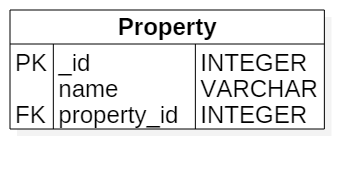
\includegraphics[width=6cm]{images/ERProperty.png} 
	\caption{- ER Diagram Project Property} 
	\label{fig:erproperty}
\end{figure}\\
Figure \ref{fig:plproperty} describes the \textit{ER diagram} for the programming language property concluding the tables for conversion costs and language properties. This is described in this section as an example of properties. The complete entity relation diagram can be found in the appendix XXX. As described above the table \textit{ProgrammingLanguage} contains and \textit{\_id} column and a column with the \textit{name} of the programming language. The column \textit{property\_id} is a foreign key and is a reference to the table \textit{ProgrammingLanguageProperty}. This table contains the properties of a programming language as described in section \ref{section:ProgrammingLanguage}. The table \textit{ProgrammingLanguageConversionCosts} contains the previous calculated costs for converting source code from one programming language to another.  
\begin{figure}[h] 
	\centering 
	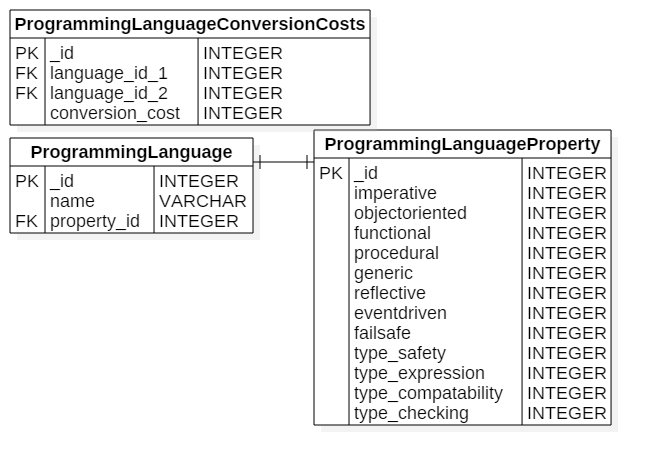
\includegraphics[width=10cm]{images/PLProperty.png} 
	\caption{- ER Diagram Project Property} 
	\label{fig:plproperty}
\end{figure}\\

\subsubsection{Projects}

The data of projects is stored in several tables. As described in figure \ref{fig:projectER} these tables are named \textit{Project}, \textit{ProjectDetails}, \textit{EstimationTechnique} and \textit{ProjectProperty}. Also the tables \textit{FunctionPointInfluenceFactor}, \textit{FunctionPointEstimation} and the estimation item tables, here portrayed as the table \textit{InputData} are important for an estimation with function point.\\
The \textit{EstimationTechnique} table stores all available techniques for projects. It contains only the id and name of a technique. The \textit{Project} table itself contains the selected estimation technique as a foreign key. As described in fig. \ref{fig:projectER}, the connection between EstimationTechnique and Project is a many-to-one connection. A project can only have one estimation technique, but a estimation technique can be used by many project. Further columns are the name of the project and the creation date in the column \textit{created\_at}. The column \textit{is\_deleted} is a flag to state if the project was already deleted. Also the column \textit{is\_terminated} stands for the termination of a project. The last column is the \textit{project\_detail\_id} which is also a foreign key to the table \textit{ProjectDetails}. The connection here is a \textit{one-to-one} relation. This table mainly contains foreign keys to other tables but for the estimation and influence factors it is not possible to set foreign keys. This depends on the selected estimation technique and selection of the right table is made in the implementation which is described at section \ref{impl:estMethodSelection}. The column \textit{evaluated\_person\_days} stores the amount of days the estimation technique calculated for a project. To load the right project icon the column \textit{icon\_id} refers to the table \textit{ProjectIcons}, which stores name and path of an icon. How this icon is loaded is described in section \ref{impl:loadProjectIcons}. As descriptions can be a long \texttt{string}, they are stored in an extra table called \textit{ProjectDescription}. This is made for a better overview of the \textit{ProjectDetails} table. The last foreign key in \textit{ProjectDetails} refers to the table \textit{ProjectProperty}. It contains the id of selected properties for a project.\\
The estimation itself depends on the selected estimation technique. In this paper only the \textit{Function Point} technique is implemented and described. The estimation itself is stored within the \textit{FunctionPointEstimation} table. It contains foreign keys to the estimation items for each category. Each of this tables is structured the same as the described \textit{InputData} table. It contains the \textit{\_id}, simple, medium and complex value of a category. The other important table is \textit{FunctionPointInfluenceFactor}. All influence factors as described in section \ref{fp:classificationInfluence} are stored here.
\begin{figure}[h] 
	\centering 
	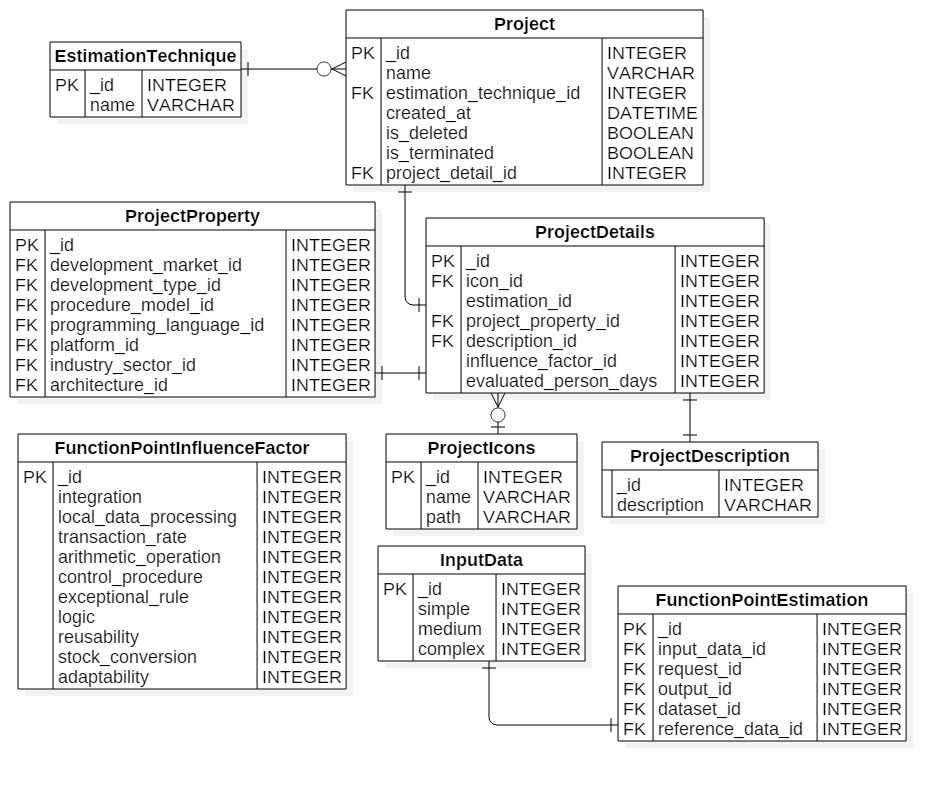
\includegraphics[width=13cm]{images/projectDiagramm.png} 
	\caption{- Entity Relation Diagram  for Project Informations} 
	\label{fig:projectER}
\end{figure}

\subsection{Userinformation Database}

This database was designed for future use of a server connection. The \textit{User} table stores the information of an authorized user on the device. It contains \textit{name}, \textit{password} and \textit{mail} address to identify a user. Also the column \textit{device\_id} gives information of the device he is using. The \textit{MessageQueue} table stores all messages that where synchronized from the server. This contains for example updates for the project properties.
\begin{figure}[h] 
	\centering 
	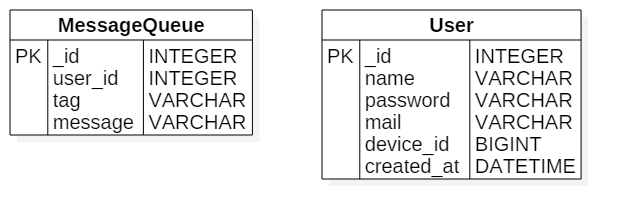
\includegraphics[width=14cm]{images/userDBDiagramm.png} 
	\caption{- Entity Relation Diagram  for User Informations} 
	\label{fig:userER}
\end{figure}

\section{User Interface}

This chapter describes the user interface design.

\subsection{Projects Overview}

Anordnung der Projekte, Wichtige Informationen zum sehen, Filtern und Suchen nach Projekten

\subsection{Project Creation}

Komponente zur korrekten Erstellung von Projekten, Geführte Eingabe, Korrekte Erstellung von Projekten in der DB, Swipe Funktion

\begin{figure}[h] 
	\centering 
	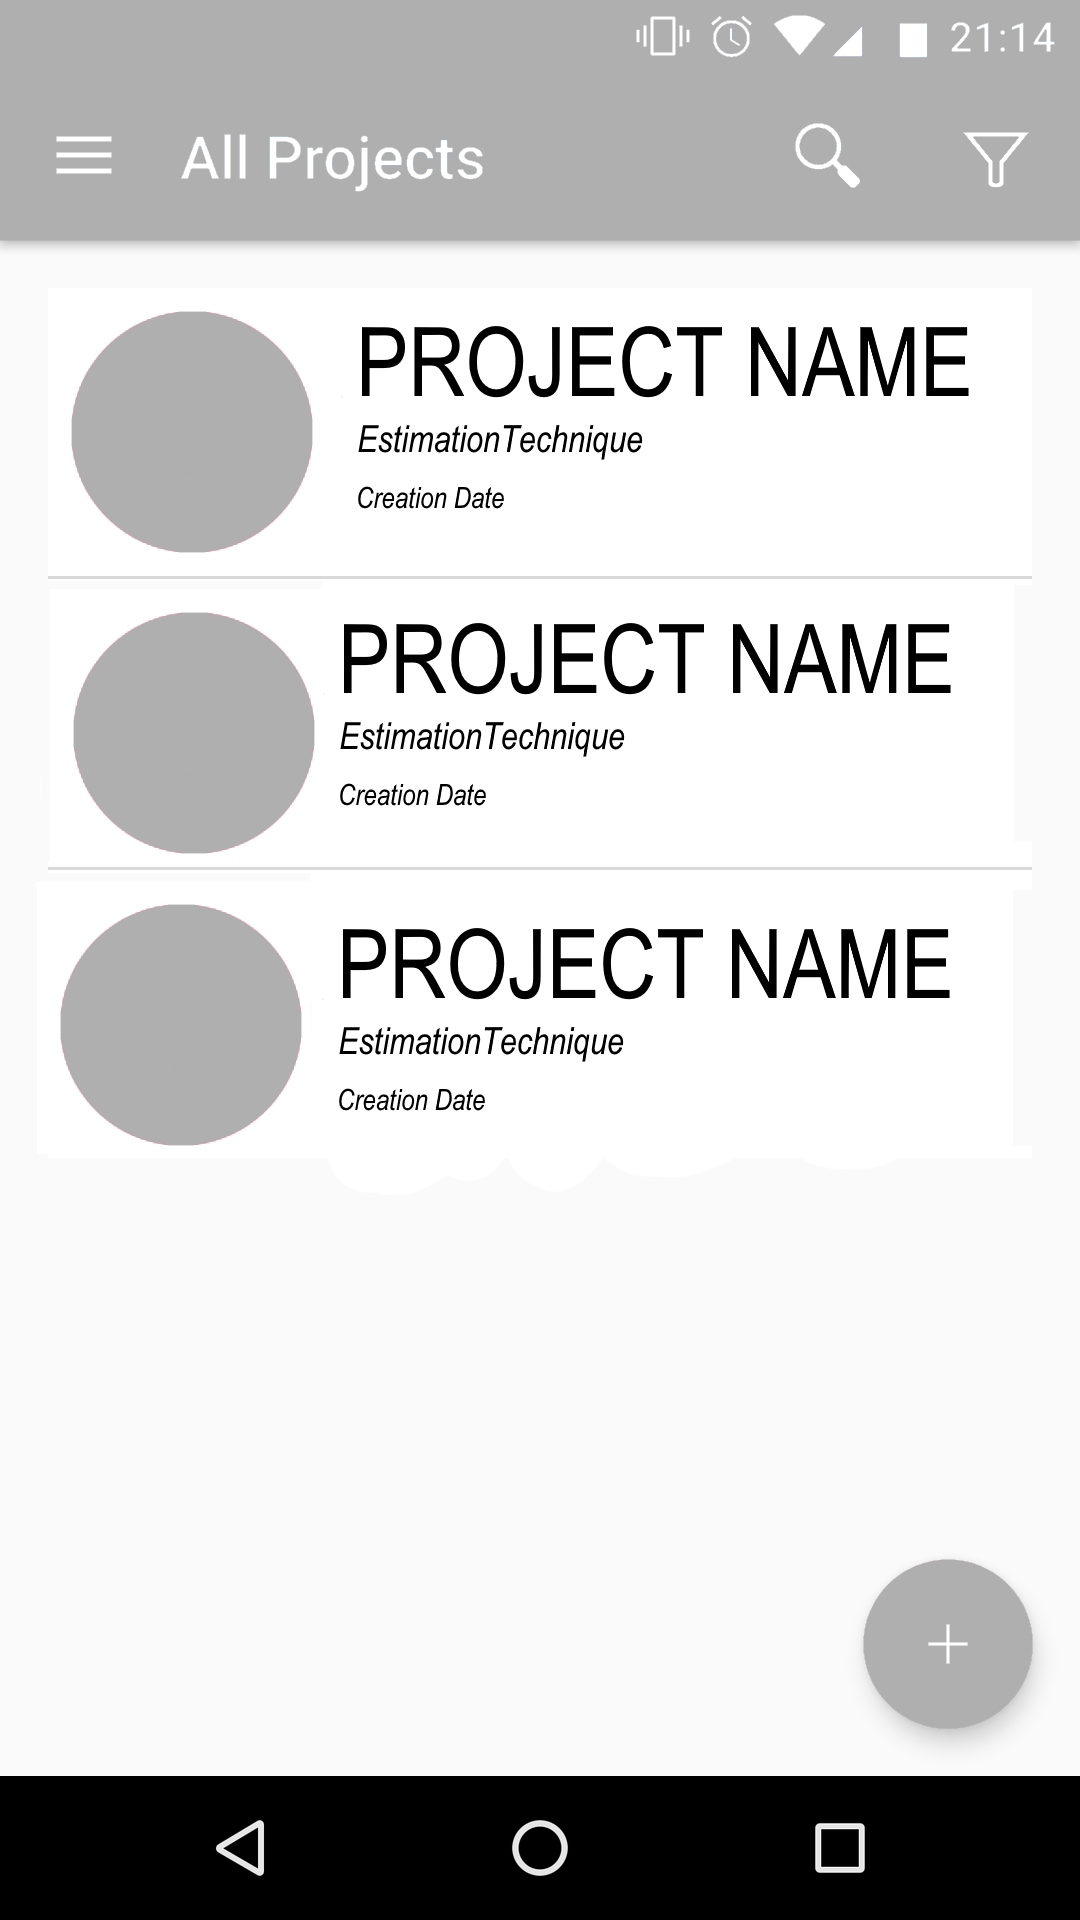
\includegraphics[width=6cm]{images/projectoverview.png} 
	\caption{- Entity Relation Diagram  for User Informations} 
	\label{fig:fpcreate}
\end{figure}

\subsection{Estimate Function Point Project}

Aufbau der Schätzung, Umwandlung von Tabelle in App

\subsection{Influence Factors}

Aufbau der EInflussfaktoren, Neue anlengen

\subsection{Analysis}

Wie die Analyse aufgebau und was soll diese bringen?

\section{Adjusted Estimation Process}\label{adjustedEstimationProcess}


\subsection{Continuous Improvement of the Estimation}

